\vspace{0.5cm}
\begin{center}
    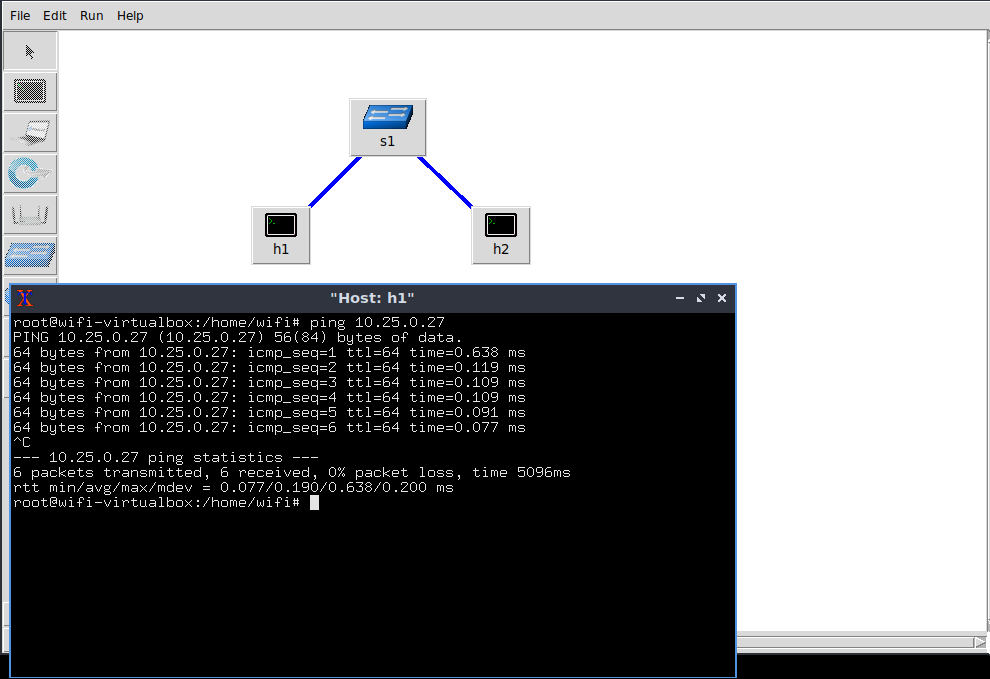
\includegraphics[width=1\textwidth]{./images/T1.2TopologyAndPing.png}
\end{center}
\textbf{1:} `tc qdisc add dev h2-eth0 root netem rate 125mbit`
\begin{center}
    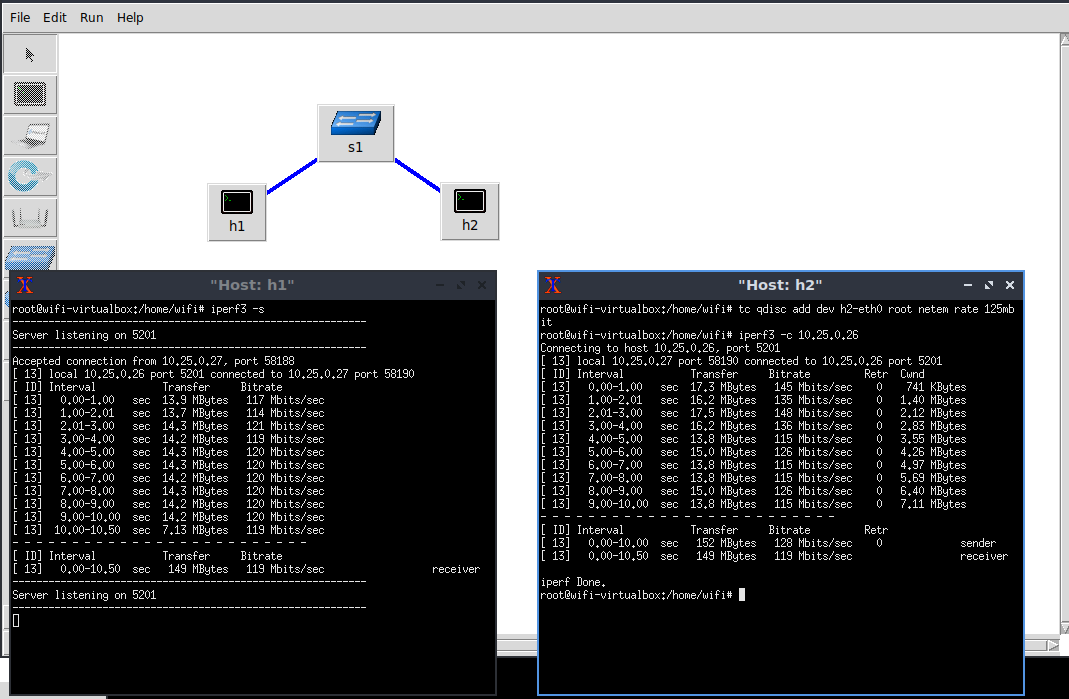
\includegraphics[width=1\textwidth]{./images/T1.2/125test2.png}
    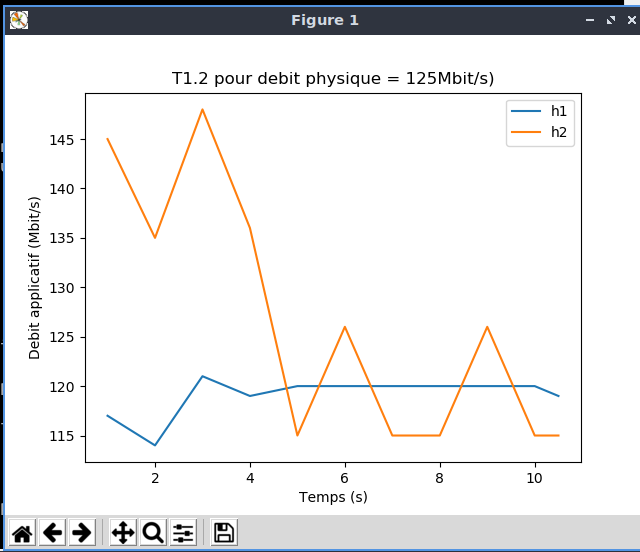
\includegraphics[width=1\textwidth]{./images/T1.2/courbe125test2.png}
    
\end{center}
\textbf{Observation :}\\
Débit de H1 (ligne bleue) : Le débit applicatif mesuré sur h1 reste relativement stable, oscillant entre 115 Mbit/s et 125 Mbit/s tout au long du test. Même si le lien physique entre H1 et le switch est de 1 Gbit/s, le débit observé n’atteint jamais cette valeur maximale théorique.

Débit de H2 (ligne orange) : Le débit applicatif de H2 fluctue considérablement, atteignant parfois des pics autour de 145 Mbit/s, mais chutant aussi à des valeurs proches de 120 Mbit/s ou même légèrement en dessous.
\vspace{1cm}
\\
\textbf{Explications :} 
\\
Bien que la liaison entre h1 et le switch soit fixée à 1 Gbit/s, c'est le lien entre H2 et le switch qui impose une limite plus contraignante de 125 Mbit/s.\\
Dans ce type de configuration, le débit total du transfert est dicté par le maillon le plus faible de la chaîne, en l’occurrence la connexion limitée entre H2 et le switch. Le lien de 1 Gbit/s entre h1 et le switch ne peut donc pas être exploité pleinement tant que H2 ne peut pas recevoir ou envoyer des données plus rapidement que 125 Mbit/s.\\
\\
L'outil iperf3 utilise généralement le protocole TCP, qui ajuste automatiquement le débit en fonction des capacités du réseau. TCP surveille les capacités des deux hôtes et ajuste son débit en fonction des retours qu’il reçoit (accusés de réception des paquets).
Ici, TCP détecte que le débit sur le lien entre H2 et le switch est limité à 125 Mbit/s et ajuste donc la transmission des données pour s’adapter à cette contrainte, expliquant pourquoi le débit de h1 reste autour de 115 à 125 Mbit/s.
Le protocole TCP est conçu pour éviter la surcharge du réseau et s’adapte dynamiquement aux conditions de congestion, ce qui pourrait aussi expliquer pourquoi le débit de H2 est plus instable, car le lien est proche de sa capacité maximale.\\
\\
\textbf{2:} `tc qdisc add dev h2-eth0 root netem rate 625mbit `
\begin{center}
    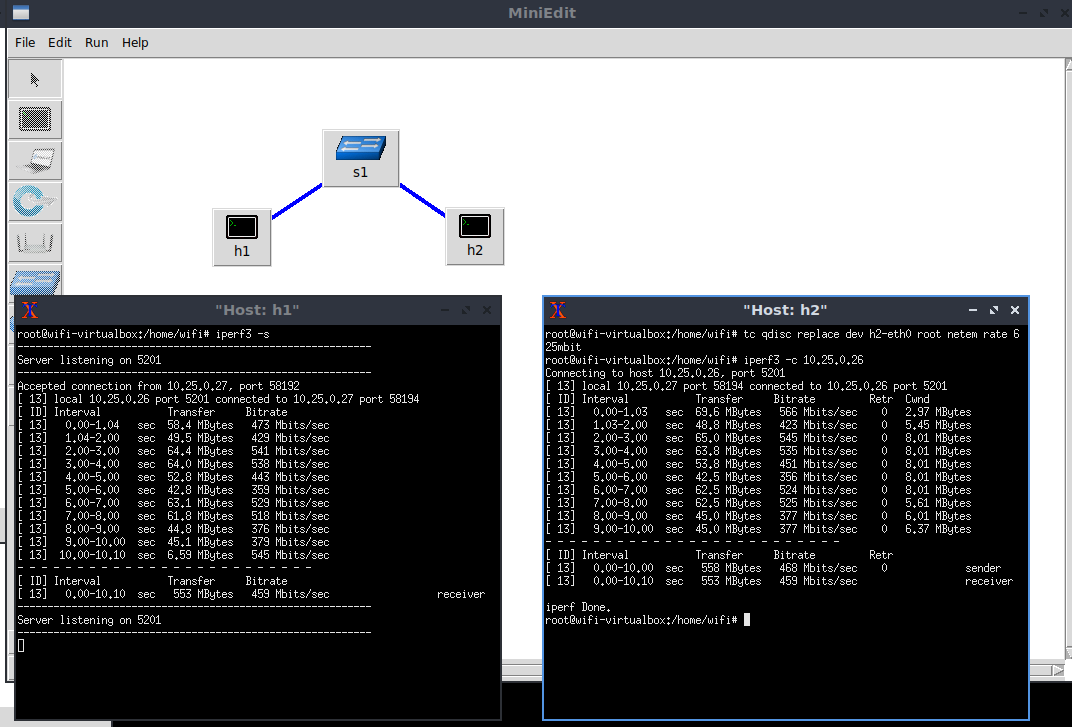
\includegraphics[width=1\textwidth]{./images/T1.2/625test2.png}
    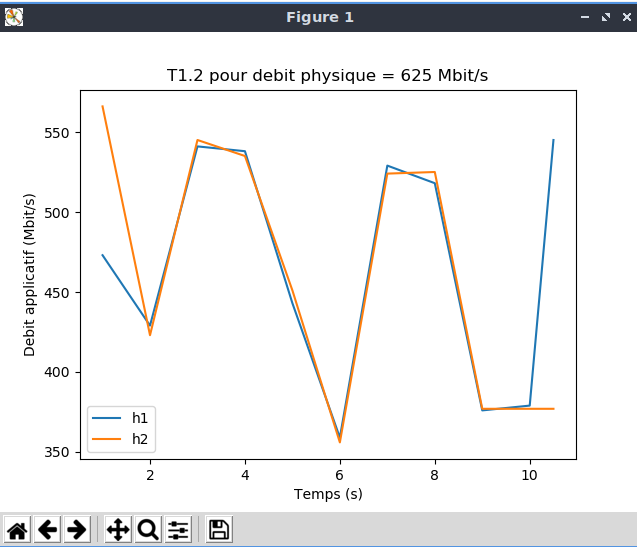
\includegraphics[width=1\textwidth]{./images/T1.2/courbe625test2.png}
\end{center}
\textbf{Observation :}\\
Débit de h1 (ligne bleue) : Le débit applicatif mesuré sur h1 varie entre 350 Mbit/s et environ 550 Mbit/s.
Débit de h2 (ligne orange) : Le débit applicatif sur H2 suit une courbe similaire à celle de h1.
\\
\\
\textbf{Explication} :\\
Le fait que les deux débits (h1 et h2) suivent un schéma similaire de montée et descente suggère que la limitation du débit physique à 625 Mbit/s entre H2 et le switch influence directement les deux hôtes. Comme le débit de H2 est limité par le lien physique, le switch agit comme un point de congestion, entraînant des fluctuations du débit applicatif.
\vspace{1cm}
\\
\newpage
\textbf{3:} `tc qdisc add dev h2-eth0 root netem rate 2.5gbit`
\begin{center}
    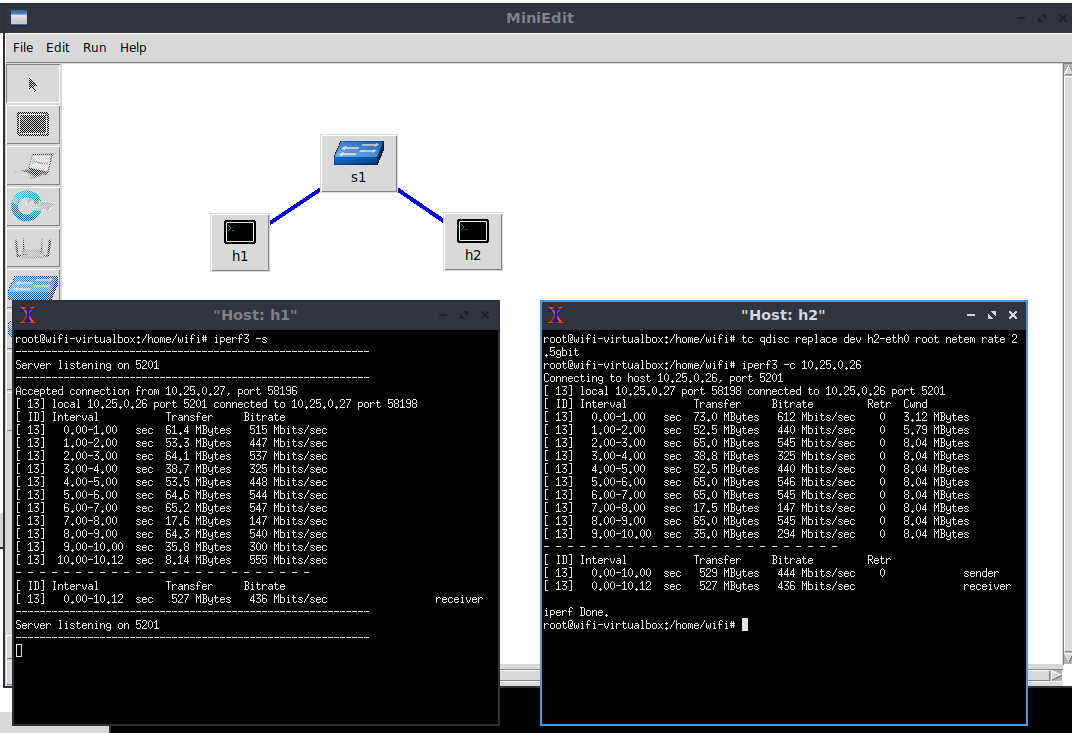
\includegraphics[width=1\textwidth]{./images/T1.2/2500test2.png}
    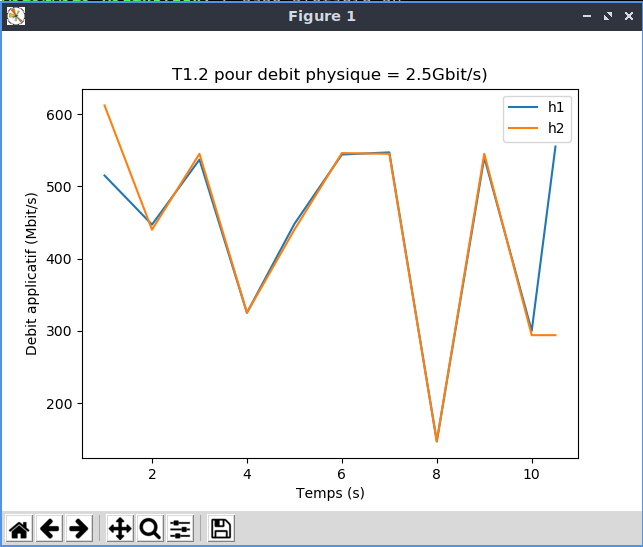
\includegraphics[width=1\textwidth]{./images/T1.2/courbe2500test2.png}
\end{center}
\textbf{Explication} :\\
Le débit applicatif oscille de manière significative entre environ 100 Mbit/s et 600 Mbit/s sur la période mesurée (10 secondes).
\\

Les courbes de h1 et h2 sont très proches, ce qui indique une synchronisation des débits mesurés sur les deux hôtes.`\\
Le fait de fixer le débit de l'interface h2 à 2.5 Gbit/s alors que le lien entre h1 et le switch est limité à 1 Gbit/s signifie que le débit maximum théorique du transfert sera contraint par cette limite de 1 Gbit/s.
\\
\\Toutefois, les fluctuations observées montrent que le débit applicatif est souvent bien en-dessous de ce maximum théorique, probablement en raison des phénomènes de contention et de gestion des files d'attente (dqisc).
\vspace{0.5cm}
\\
Si le lien entre h1 et le switch est limité à 1 Gbit/s, alors que le lien entre h2 et le switch peut aller jusqu'à 2.5 Gbit/s, il y a un déséquilibre.
Lorsqu'h2 essaie d'envoyer des données à un débit supérieur à 1 Gbit/s, le switch doit gérer cette surcharge, créant ainsi une contention pour la bande passante disponible.
\\
En présence de forte contention, des collisions peuvent se produire (particulièrement sur les réseaux partagés comme Ethernet en mode half-duplex).
Les paquets peuvent être perdus et doivent être retransmis, ce qui réduit l'efficacité du débit applicatif.



\newpage
\section{Comparaison des Tests T1.1 et T1.2}


\subsection{Résultats pour un Débit Physique de 125 Mbit/s}
\begin{center}
    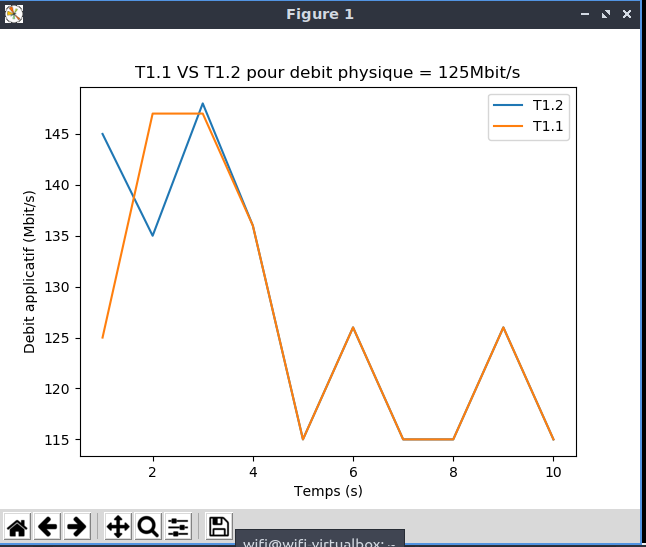
\includegraphics[width=1\textwidth]{./images/T1vsT2pour125.png}
\end{center}
\textbf{Analyse :}\\
\textbf{Débit Initial :} T1.2 affiche un débit initial plus élevé (environ 145 Mbit/s) par rapport à T1.1, qui démarre autour de 125 Mbit/s.\\
\textbf{Pic de Débit :} Les deux configurations atteignent un pic de débit d'environ 145 Mbit/s entre 2 et 3 secondes, mais T1.1 atteint son pic légèrement avant T1.2.\\
\textbf{Stabilité et Fluctuations :} T1.2 montre des fluctuations significatives après le pic, tandis que T1.1 reste plus stable au départ avant de fluctuer également.\\
\textbf{Conclusion (125 Mbit/s) :} T1.2 est initialement plus stable, mais les deux configurations montrent une instabilité après quelques secondes.

\subsection{Résultats pour un Débit Physique de 625 Mbit/s}
\begin{center}
    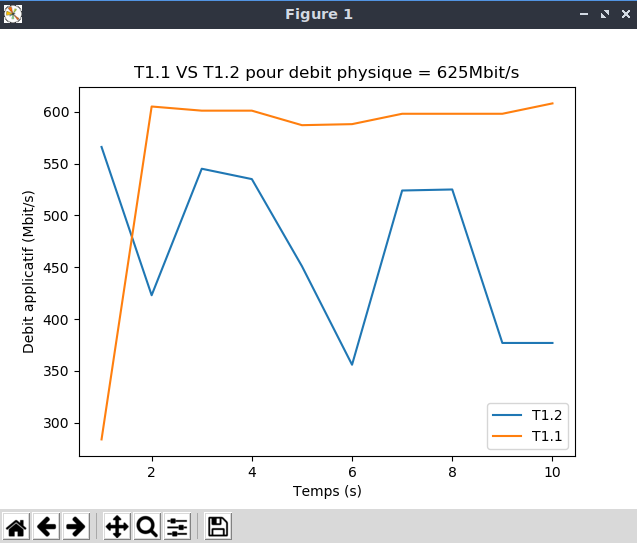
\includegraphics[width=1\textwidth]{./images/T1vsT2pour625.png}
\end{center}
\textbf{Analyse :}\\
\textbf{Comportement Initial :} T1.1 atteint rapidement environ 600 Mbit/s et reste stable, tandis que T1.2 montre des fluctuations initiales, atteignant environ 550 Mbit/s.\\
\textbf{Stabilité et Consistance :} T1.1 est stable et proche de la limite physique, tandis que T1.2 est instable, avec des variations importantes.\\
\textbf{Conclusion (625 Mbit/s) :} Le lien direct (T1.1) offre une performance supérieure, avec un débit plus stable.

\subsection{Interprétation des Résultats pour un Débit Physique de 2,5 Gbit/s}
\begin{center}
    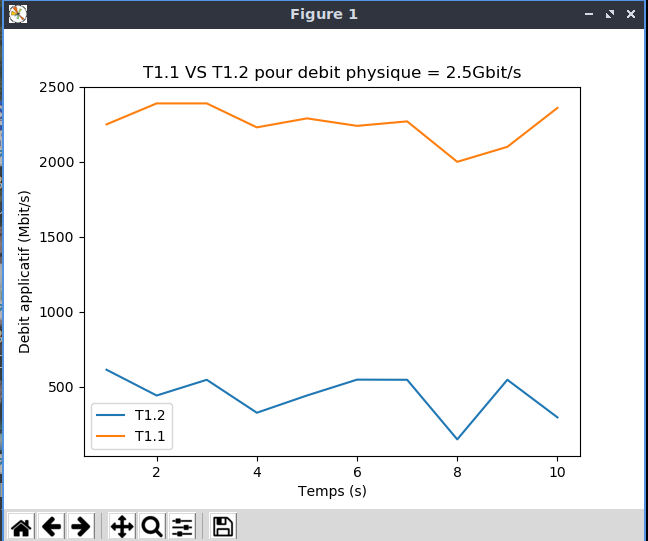
\includegraphics[width=1\textwidth]{./images/T1vsT2pour2500.png}
\end{center}
\textbf{Analyse :}\\
\textbf{Performance du Lien Direct (T1.1) :} Le débit est proche de 2,4 Gbit/s, montrant une communication très efficace.\\
\textbf{Performance avec le Switch (T1.2) :} Le débit fluctue autour de 600 mbit/s, indiquant des délais de traitement et une surcharge du switch.\\
\textbf{Conclusion (2,5 Gbit/s) :} Le lien direct est plus performant à des débits élevés, tandis que l'ajout d'un switch entraîne une dégradation notable du débit.

\subsection{Interprétation Finale et Conclusion}
\textbf{Impact de la Topologie du Réseau :}\\
\textbf{Lien Direct (T1.1) :} Offre une meilleure performance, minimisant les latences et maximisant l'utilisation du débit physique.\\
\textbf{Switch (T1.2) :} Introduit une surcharge, réduisant la performance, surtout à des débits élevés.\\
\textbf{Conclusion Générale :}\\
Pour des applications nécessitant un débit élevé et constant, une connexion directe est préférable. L'utilisation d'un switch est recommandée pour des scénarios nécessitant flexibilité et expansion du réseau, bien qu'elle puisse entraîner des baisses de performance. En résumé, le choix de la topologie doit être basé sur les exigences de l'application, en équilibrant performance et flexibilité.